\chapter{Introduction}
\label{chap:introduction}

%-----------------------------------------------
%  GENERAL CONTEXT
%-----------------------------------------------
\section{General context}

\subsection{Human hearing}

\lettrine{W}{e}, as humans, have been granted a couple of ears capable of reacting to surrounding sound and processing the vibrations through our brain. From even before our birth, we have learned to use them properly, and we have impressive capabilities of dealing with a complex sound environment.

Imagine yourself at a friend's party. Many guests are present, you are in the middle of a discussion with two friends, surrounded with other small groups of chatting people. A few meters from you, one of the guest performs an entertaining dub music DJ set, while someone is ringing at the door. A lot of audio information arrive at the same time to your ears. Yet, you are still able to understand what your two friends are debating, and you can handle the conversation, maybe at the cost of speaking louder. Also, you can shift your attention at any time by indiscreetly listening the next group's conversation, or enjoying the music coming from the DJ booth, while being aware that a new guest is arriving at the door. This phenomenon is called the \textit{cocktail party effect} \cite{arons_review_1992}. It refers to the brain's ability to let us focus on any sound stimulus among many other stimuli. In other words, the fact that all sounds are mixed together when incoming to our ears is not an obstacle for us to understand the surrounding sound space.

The cocktail party effect is partially due to our great ability for sound source localization. Because our ears do not receive the exact same sound signal at a given instant, the brain can sense small differences in intensity, spectral content and timing cues between the two signals in order to locate the sound sources \cite{bregman_auditory_1994}. Except if a sound source location is equidistant to both ears, the signals arrive time-shifted from each other and this time difference is a localization cue. The shapes of our head, torso and pinna cause diffraction which also helps to locate sound sources \cite{blauert_spatial_1997}. Consequently, all human beings perceive sound differently, and we have learned to hear based on the characteristics of the body parts around our ears. We are also capable of estimating the source distance based on the loss of amplitude and the ratio between the direct path and the reverberated part. Thus, our localization ability is greatly responsible for our capacity to extract meaningful information from a complex sound environment.

\subsection{What is sound ?}

Sound is a vibration travelling through a medium. It propagates, as a wave, in any medium allowing local oscillations: gases, fluids and solids. On Earth, silence almost does not exist. Any vibrating object, like flowers, tree leaves, fleas, fish, wind, icebergs, underwater volcanoes, loudspeaker, guitar string, emits a sound wave and acts as a sound source. The resulting vibration then freely travels through the surrounding medium, if no obstacle is encountered, at a speed $c$ depending on the medium properties (in the air, $c = \SI{343}{\meter\per\second}$ at $\SI{20}{\degreeCelsius}$). When a sound wave passes through a fixed point in space, local pressure and velocity vary in time, a little shifted from the equilibrium state. The changes are generally very small. On Earth, the average atmospheric pressure at the surface is around $100\,000$~Pa, while the just audible pressure deviation for human hearing is $0.00002$~Pa (corresponding to $0$~dB in sound pressure level, SPL), and the threshold of pain is between $20$ and $200$~Pa (corresponding to $120$-$140$~dB SPL). 

In such a vibrating phenomenon, frequency is defined as the number of vibrations per second, or \textit{Hertz} (Hz). In nature, most sound waves are propagating vibrations containing multiple frequencies, which characterize its  aspect, commonly referred as \textit{timbre}. For example, a guitar bass sound is mainly made of \textit{low} frequencies, whereas a singing bird mostly emits \textit{high} frequencies. We can describe a complex wave (\emph{i.e.}, containing many frequencies) in terms of a superposition of sinusoidal plane waves, each one containing only one frequency. As a sound source vibration evolves with time (for instance, it can attenuate), its frequency content also evolves. Thus, the time and frequency dimensions are two important characteristics of a sound wave.

When a sound wave encounters an obstacle, several phenomena can occur. \textit{Specular reflections} happen when the wave arrives at a smooth surface, like a wall. In this case, the incoming sound wave is reflected in the opposite direction from the wall, at an angle equal to the incoming angle. When the irregularities of a surface are smaller than the wavelength -- the distance over which a wave's shape is repeated - we witness \textit{scattering}, whose consequence is a propagation of the incoming wave into directions deviated from a straight trajectory. Another phenomenon, \textit{diffraction}, can occur when the wave passes across a surface edge.

As sound waves cause local displacements of matter (vibrations) when travelling through a medium, they obey the superposition principle. That is, when two sound waves incoming from two separated sound sources pass through the same point in space, the vibrations are added, resulting in a combination of the propagated information, as illustrated in Fig.~\ref{fig:superpositionPrinciple}. This property makes the analysis of sound complicated: when recording the surround sound scene with one or several microphones, it is not straightforward to decompose the different incoming sound waves according to their respective source.

\begin{figure}[t]
    \begin{center}
    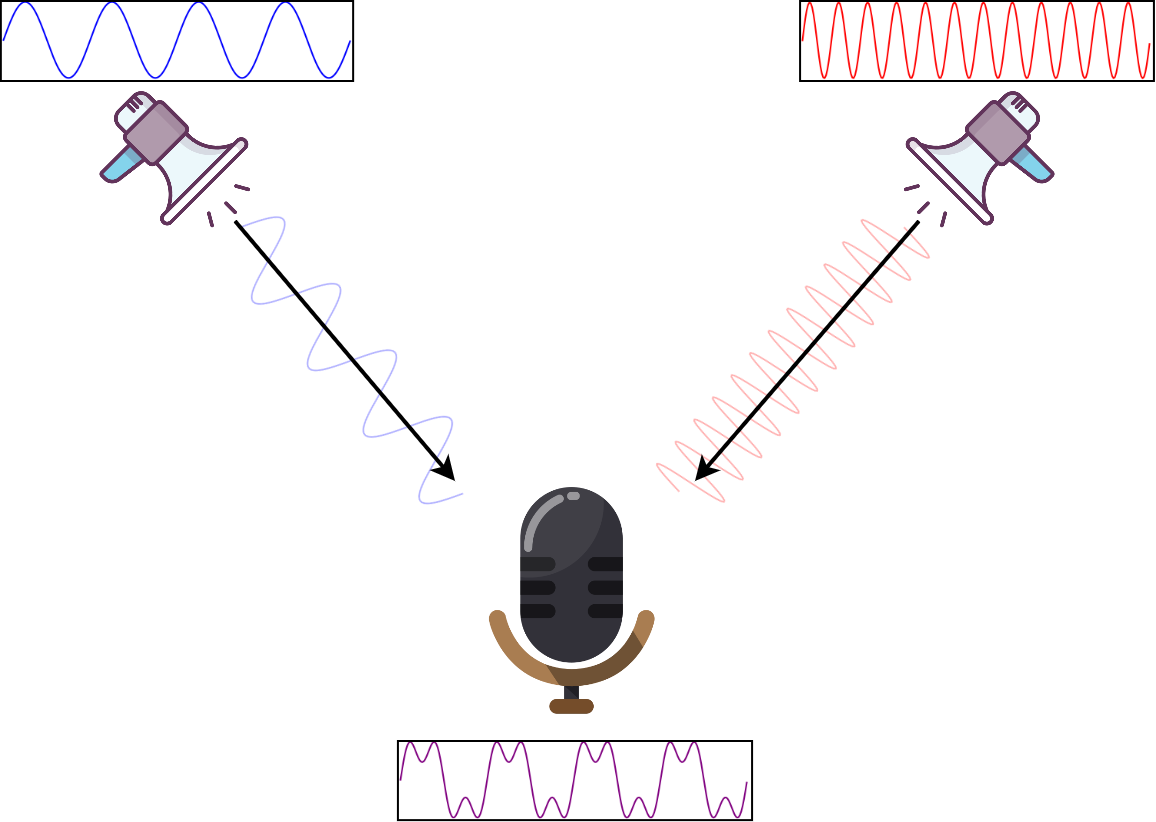
\includegraphics[width=0.7\linewidth]{Images/chap1/superpositionPrinciple.png}
    \captionof{figure}[Superposition of two sound waves]{Superposition of two sound waves arriving simultaneously at the same point in space. The signal in purple, recorded by the microphone, is the sum of the two incoming sound signals, in blue and red. The black arrows illustrate the propagation of the waves from the sound sources to the microphone.}
    \label{fig:superpositionPrinciple}
    \end{center}
\end{figure}

This phenomenon is even more accentuated when a sound wave propagates in an environment with walls and furniture. As illustrated in Fig.~\ref{fig:multipathPropagation}, the sound wave can reflect successively multiple times onto the walls, following a determined path. Moreover, as most sound sources generate spherical waves, leading to a spherical wavefront, the wave propagates in many directions at the same time (illustrated by the multiple arrows coming from the loudspeaker in Fig.~\ref{fig:multipathPropagation}). Because of the many resulting reflections, several delayed copies of the same wave arrive simultaneously at the recording point. Due to the superposition principle, they are added together to the \textit{direct path}, which is the wavefront going directly from the sound source to the receiver. The resulting recorded signal is thus not an exact copy of the original source signal, but rather a combination of delayed and attenuated versions of the original signal. The phenomenon of a signal coming to a receiver from several paths is called \textit{multipath propagation}. The first reflections form what is called \textit{early reflections}, which generally lasts a few milliseconds, until there are ``too many'' of them, which is referred as \textit{reverberation}. Reverberation happens in every closed space, and is more or less accentuated depending on several parameters, such as wall materials or room dimensions. Typically, high reverberation can be heard in churches and cathedrals, while special rooms called \textit{anechoic chambers} have been designed to minimize the effect of reverberation.

\begin{figure}[t]
    \begin{center}
    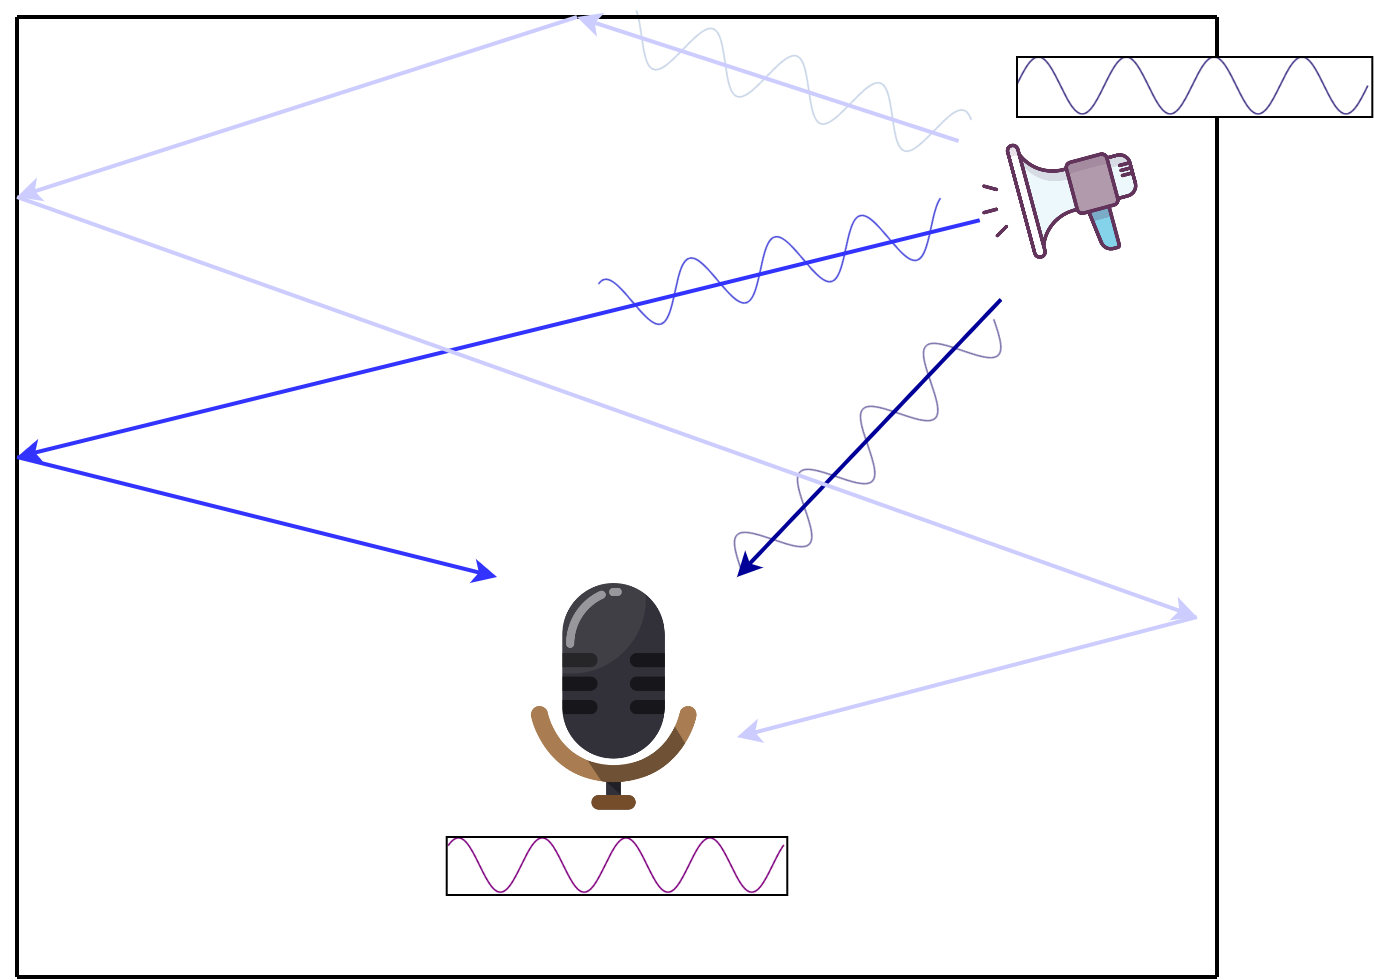
\includegraphics[width=0.6\linewidth]{Images/chap1/multipathPropagation.png}
    \captionof{figure}[Multipath propagation]{Illustration of a multipath propagation, which occurs in the presence of walls where the wavefront of a single sound wave reflects several times onto. The dark blue arrow exhibits the \textit{direct path} from the source to the receiver, and the two other arrows show two different paths that do not arrive at the same time as the direct path. The resulting recorded signal is a combination of all the received waves, delayed from each other because of different path lengths.}
    \label{fig:multipathPropagation}
    \end{center}
\end{figure}

As we can see, the superposition principle makes it difficult to retrieve a clean version of the original sound source signal in a real-world environment. When several sources occur, or when there are reflections in a room, the fact that different sound waves arrive at the recording point makes it very difficult to retrieve the original signals without prior information.


\subsection{Audio signal processing}

For decades, researchers have been trying to reproduce the human hearing abilities using machines. The general motivation of this research effort is to build systems capable of understanding the surrounding sound scene. Such systems require one or more microphones, mimicking the human ears, and signal processing algorithms replacing the brain activity. To accomplish certain goals, usually several algorithms are interconnected into a processing chain, such that each one performs a specific subtask, in order to form a fully-working system. Let us take the example of a system capable of decoding human speech, commonly named automatic speech recognition (ASR) \cite{nassif_speech_2019}. If one can record a perfectly clean speech signal, directly applying an effective ASR algorithm might be sufficient. But in a real-world context, a lot of interference makes the task more complicated. For example, in a domestic environment, other sources (dog barks, TV sound, vacuum cleaning, etc.) could interfere with the target speech signal, as well as surrounding noise coming for example from the outside of an open window. Reverberation is also an important factor that blurs the original speech signal.

To cope with this challenging conditions, several audio signal processing algorithms can be used to clean the recorded speech signal beforehand. As their names refer, \textit{denoising} and \textit{dereverberation} algorithms, often encapsulated as \textit{speech enhancement} \cite{vincent_audio_2018}, aim to remove or at least reduce noise interference and reverberant parts of a signal, respectively. When several sound sources are captured, \textit{source separation} \cite{wang_supervised_2018} aims to separate a mixture signal into several component signals, each one containing the information coming from a single particular source. Source separation techniques can rely on frequency contents, or be obtained by spatial filtering when multiple microphones are used. In the latter type of methods, assuming the knowledge of the target source location, one can spatially filter out the unwanted part of the sound field and extract the sound coming from the target location. However such methods rely on the knowledge of the source location(s), which can be estimated using \textit{sound source  localization} (SSL). To estimate the source(s) location, one needs at least two microphones. SSL algorithms can estimate the directions of one or more overlapping sound sources, and a \textit{source counting} method might be handy to apply beforehand, to ensure that the right number of sources are located in the analyzed signal. Note that when we deal with speech signals, source counting (thus named \textit{speech counting)} is a subtask of \textit{speaker diarization} \cite{anguera_speaker_2012,tranter_overview_2006,park_review_2021}, which is the task aiming to answer the question \textit{who speaks and when ?} in a signal.

\subsection{Thesis focus}

\subsubsection{Speaker counting and localization}
In this thesis, we addressed two of the previously mentioned audio tasks: sound source localization and source counting. More precisely, we deal with speech sources. As stated above, knowing the number of speakers in a signal is a very useful piece of information to extract beforehand. It could prevent the localization algorithm focus onto more sources than the sound really contains, and thus avoid the inclusion of interfering sources, such as noise. Part of this thesis work was thus to design an algorithm capable of counting the number of speakers in challenging acoustic conditions, \emph{i.e.}, in noisy and reverberant environments. The other focus of this thesis was to explore speaker localization in the same kind of challenging environments. Following our interest in counting speakers, we aimed to localize several overlapping speech sources. In order to design robust systems for counting and localizing multiple speakers, our research exploited several tools. 

\subsubsection{Ambisonics format}
Throughout this thesis, we took benefit of the Ambisonics format to represent the sound signal. Such a format is obtained from a spherical microphone array, leading to a multi-channel signal. This more and more adopted audio format presents several great advantages. It is agnostic to the choice of microphone array, that is the encoded signal does not depend on the arrangement of microphones within an array. The sound scene can also be rendered given any disposition of loudspeakers from this format, but this aspect was not of interest in this thesis. Also, it is an isotropic format, meaning that the recording process does not favor any direction. We detail this format in Chapter~\ref{chap:ambisonics}.

\subsubsection{Artificial neural networks}
We explored the potential of artificial neural networks to design robust sound source counting and localization systems. This family of models is part of \textit{deep learning} (DL) \cite{goodfellow_deep_2016}, which is a class of algorithms behind most recent artificial intelligence systems. Their success is due to the ability of neural networks to model complex functions by adjusting their parameters through a learning phase based on a dataset of many examples. They are more and more used today, due to the amount of available data and the increasing computational power to train the algorithms. The basics of artificial neural networks are presented in Chapter~\ref{chap:neuralNetworks}.

%-----------------------------------------------
%  PROBLEM FORMULATION
%-----------------------------------------------
\section{Problem formulation}

In this section, we formulate the problems of counting and localizing sources (regardless whether they are speech or not) in a mathematical framework. The goal is to formally describe the problem we address in this thesis, as well as set the notations we use throughout the chapters. 

\subsection{Mixture model}

We adopt the same mixture model formalization as in \cite{vincent_audio_2018}. Let us assume an environment with $J$ point sources, in which we place a microphone array consisting of $I$ microphones. Each microphone records the sound scene in terms of pressure change from a different position in space, resulting in a multi-channel mixture signal $\mathbf{x}(t)$ containing the recorded signal $x_i(t)$ from each microphone $i$:
\begin{equation}
    \mathbf{x}(t) = \begin{bmatrix} x_1(t) \\ x_2(t) \\ \vdots \\ x_I(t) \end{bmatrix},
\end{equation}
where $t$ denotes discrete time.

As multiple sound sources are present in the environment, according to the superposition principle, each microphone signal is a sum of the signals arriving at the microphone position from each sound source $j$:

\begin{equation}
    x_i(t) = \sum_{j=1}^J c_{ij}(t).
\end{equation}

Here, $c_{ij}(t)$ is the signal arriving at microphone $i$ resulting from the emission of a signal $s_j(t)$ from sound source $j$. The propagation of the source signal and the reverberation of the room has to be taken into account. This can be modeled using a linear time-invariant filter $a_{ij}(\tau)$ if the sources and microphones are static. As all the microphones and sources are at different positions, all filters $a_{ij}$ are distinct. The signal arriving at microphone $i$ can then be expressed as:

\begin{equation}\label{eqSRIR}
    c_{ij}(t) = \sum_{\tau=0}^{+\infty} a_{ij}(\tau) s_j(t-\tau),
\end{equation}
considering a causal filter (\emph{i.e.}, depending only on past and present inputs).
The filters $a_{ij}(\tau)$ are called \textit{room impulse responses} (RIRs) and model the propagation of the source signal from the sound source position to the microphone position, including the reverberation phenomena. The reverberation components are dependent of the source and microphone positions, as well as the room properties (geometry and dimensions, material properties, etc.). Theoretically, a room impulse response is the signal recorded by a perfect microphone (without any noise), coming from a point source emitting an impulse (Dirac distribution), hence the name \textit{room impulse response}.

In real-world environment, noise is an important component which has to be included in the model of the multi-channel mixture signal. Two types of noise can be present in such a recording. On the one hand, we have to take into account the ambient noise which almost always exists in any sound scene. Such a noise is generally considered as a \textit{diffuse source}, which is a source emitting from a whole region in space, as if it was composed of an infinite number of point sources. Examples of diffuse sources include surrounding musical ambience, outside construction works, incomprehensible background conversations (usually referred to as \textit{babble noise}), or even small fluctuations of air. Such diffuse noise can be considered independent of the position in the room, thus common to all microphones. On the other hand, noise modelling the imperfection of each microphone also constitutes an important artifact. Practically, the microphones do not record the world perfectly as it is, and they are not rigorously identical to each other. Therefore, we can incorporate a noise signal $n_i(t)$ for each microphone, including both diffuse noise and microphone-wise noise, to complete the multi-channel mixture signal model:

\begin{equation}
    x_i(t) = \sum_{j=1}^J \sum_{\tau=-\infty}^{+\infty} a_{ij}(\tau) s_j(t-\tau) + n_i(t).
\end{equation}

\subsection{Room impulse responses}

The room impulse responses $a_{ij}(\tau)$ represent the acoustic behavior of the sound according to the emitting and recording positions, as well as the propagation effects induced by the presence of walls or furniture. 

Fig.~\ref{fig:impulseResponse} shows an illustration of a typical RIR. The first and highest peak (in red) represents the \textit{direct path}, which is the straight propagation between the point source and the microphone. The following peaks (in green) are referred to as \textit{early echoes} and encode the beginning of multipath propagation which includes the main reflections from the obstacles. The last part features the \textit{reverberation} phenomenon and results from the superposition of the many late reflections.

\begin{figure}[t]
    \begin{center}
    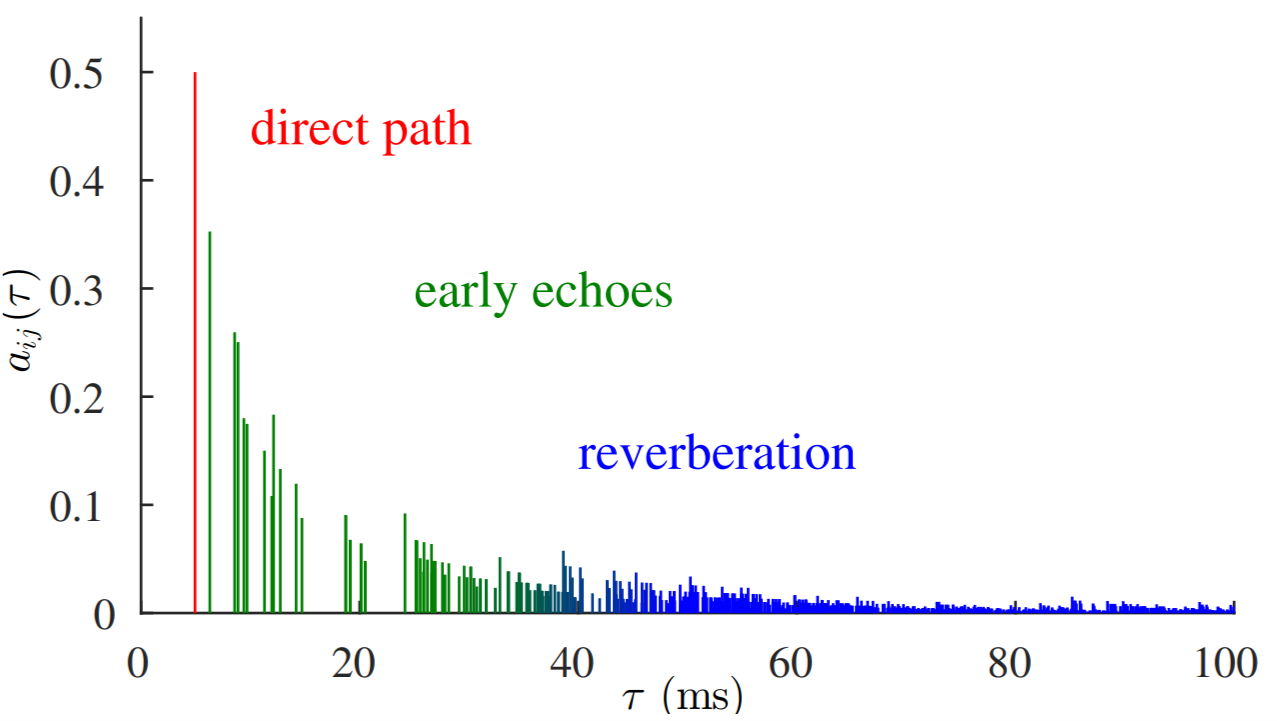
\includegraphics[width=0.6\linewidth]{Images/chap1/impulseResponse.png}
    \captionof{figure}[Illustration of an room impulse response]{Illustration of an room impulse response. Three noticeable parts in an RIR: the direct path (in red), the early echoes (in green) and the reverberation (in blue). Borrowed from \cite{vincent_audio_2018}.}
    \label{fig:impulseResponse}
    \end{center}
\end{figure}

The \textit{reverberation time} (RT60) is a quantity measuring the duration for the impulse response envelop to decrease by $60$~dB. It depends on the room size and the obstacle materials. Typical values of RT60 is between $0.2$ and $0.8$~s for small domestic rooms, and can be higher that $1$~s for larger rooms such as restaurant rooms.

\subsection{Source counting}
\label{ss:sourceCounting}

The number of sources (NoS) $J \in \mathbb{N}$ is an important piece of information which can be useful for several audio processing tasks such as source separation or source localization. For instance, knowing $J$ can improve the performance of separation or localization systems since it can help avoiding ``unwanted'' sound sources (interference). However estimating the number of sources is not straightforward, mainly due to the superposition principle. Fig.~\ref{fig:numberOfSources} illustrates the profile over time of the number of active sources in a 3-source mixture.

\begin{figure}[t]
    \begin{center}
    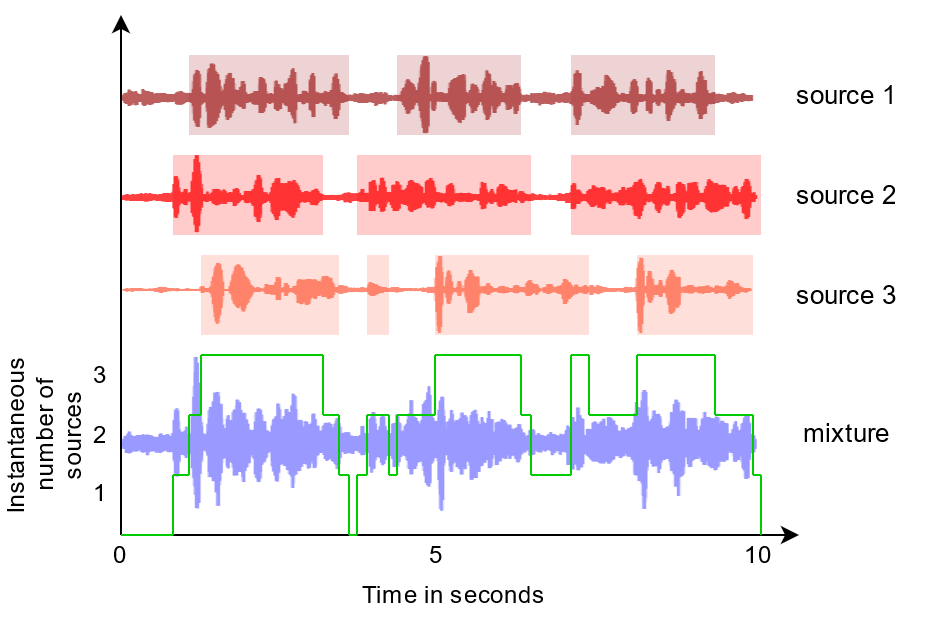
\includegraphics[width=0.8\linewidth]{Images/chap1/numberOfSources.png}
    \captionof{figure}[Example of a time profile of the number of active sources in a 3-source mixture]{Time profile of the number of active sources in a 3-source mixture. The activity of each individual source is represented with rectangles (top). The instantaneous number of active sources in the mixture $J(t)$, resulting from the superposition of each source's activity, is depicted with the green line (bottom).}
    \label{fig:numberOfSources}
    \end{center}
\end{figure}

\textit{Source counting} refers to the problem of estimating the number of sources given a single- or multi-channel mixture signal $\mathbf{x}(t)$. However this problem can be defined according to different levels of temporal resolution. The following NoS quantities can be estimated:

\begin{itemize}
    \item the instantaneous number of sources $J(t)$. The goal is to estimate the NoS at each timestep $t$, depending on the considered temporal resolution (audio sample, time frame). It is at most equal to the total NoS $J$, but it is often lower than $J$ since in general not all sources overlap at the same time;
    \item the maximum number of simultaneous sources $\bar{J}$. It is defined as $\bar{J} = \max_{t} J(t)$, which is the maximum of number of sources which were simultaneously active through the whole analyzed signal;
    \item the total number of sources $J$, which is, as previously defined, the total number of sources involved in the mixture (\textit{i.e.}, they have been active at least once during the analysis). It can be retrieved from $J(t)$ if we are able to identify the sources.
\end{itemize}

In this thesis, we were interested in estimating the instantaneous number of sources. The motivation was to provide a succeeding block in the processing chain (\emph{e.g.}, a localization or tracking algorithm) with an NoS estimate $\tilde{J}(t)$ at any time index $t$. In practice, this necessitates a source counting method operating at high temporal resolution.

Note that when $J=1$, source counting simplifies to the problem of source detection, which is predicting whether a particular source is active ($J(t)=1$) or not ($J(t)=0$) at any time $t$.

When the sources are human speakers (as it is the case in this thesis), source counting is referred to as \textit{speaker counting}, except for $J=1$ for which it is commonly named \textit{voice activity detection} (VAD). When the speech sources need to be identified in addition to counting, this problem is equivalent to \textit{speaker diarization}.

\subsection{Source localization}

The goal of SSL is to derive the spatial positions of the target source(s) based on the recorded multi-channel signal. While multiple microphone arrays can be employed to localize sources, most systems assume the use of only one microphone array, as it is a more practical solution. This problem is not trivial, notably due to the presence of noise as well as reverberation in enclosed spaces. Looking back at Fig.~\ref{fig:multipathPropagation}, we see that several signals originating from the same source arrive at the microphone from different directions. Thus, estimating the actual source direction, and even interpreting the different incoming sound waves as coming from the same point source is not a straightforward task.

Assuming an environment with $J$ emitting sources, the goal of a SSL algorithm is to estimate the position $\mathbf{r}_j(t)$ of each source $j$, given a certain coordinate system, from a multi-channel signal $\mathbf{x}(t)$. Using Euclidian coordinates, $\mathbf{r}_j(t) = (x_j(t), y_j(t), z_j(t))$, while in a spherical domain, $\mathbf{r}_j(t) = (r_j(t), \theta_j(t), \phi_j(t))$, where $r_j$ is the distance, $\theta_j$ the azimuth angle and $\phi_j$ the elevation angle. When only $\theta_j$ and $\phi_j$ are estimated, it is referred to direction-of-arrival (DoA) estimation. Spherical coordinates are especially handy when the microphone is taken as the origin. Cylindrical coordinates are used less often. 

Note that the source positions $\mathbf{r}_j(t)$ are functions of time, as in a general framework the source can be mobile in the surrounding area. In that case, sound source localization can be done with the help of a target tracking system, whose goal is to associate the multiple position estimates and the target sources over time.

%-----------------------------------------------
%  MAIN CONTRIBUTIONS
%-----------------------------------------------
\section{Main contributions}

During three thesis years, our research was focused on speaker counting and localization. Through many experiments, we explored new ways of addressing these tasks in order to improve the existing methods, and tried to analyze their behaviors. Several of these methods led to published/submitted papers:

\begin{itemize}
    \item P.-.A Grumiaux, S. Kiti\'c, L. Girin, A. Guérin, High-resolution speaker counting in reverberant rooms using CRNN with Ambisonics features, \textit{European Signal Processing Conference (EUSIPCO)}, Amsterdam, Netherlands, 2020. 
    \item P.-.A Grumiaux, S. Kiti\'c, L. Girin, A. Guérin, Multichannel CRNN for speaker counting: an analysis of performance, \textit{Forum Acusticum (FA2020)}, Lyon, France, 2020. 
    \item P.-.A Grumiaux, S. Kiti\'c, L. Girin, A. Guérin, Improved feature extraction for CRNN-based multiple sound source localization, \textit{European Signal Processing Conference (EUSIPCO)}, Dublin, Ireland, 2021. 
    \item P.-.A Grumiaux, S. Kiti\'c, P. Srivastava, L. Girin, A. Guérin, SALADnet: Self-Attentive multisource Localization in the Ambisonics Domain, \textit{IEEE Workshop on Applications of Signal Processing to Audio and Acoustics (WASPAA)}, Mohonk Mountain House, New Paltz, NY, 2021.
    \item P.-.A Grumiaux, S. Kiti\'c, L. Girin, A. Guérin, A survey of sound source localization with deep learning methods, Submitted to the Journal of the Acoustical Society of America, 2021.
\end{itemize}

\subsection{Speech counting}

We explored several neural network architectures in order to improve existing methods for speech counting. We showed that relying on multi-channel features (in the Ambisonics format) we could obtain improved speaker counting compared to using single-channel signals. Our method showed great performance to count up to $5$ simultaneous speakers in noisy and reverberant environments, at a short-term frame-wise resolution. This work was presented at the European Conference on Signal Processing in 2020 \cite{grumiaux_high-resolution_2020}. We also conducted several analyses on the performance of neural network architectures according to different hyperparameters, leading to a presentation \cite{grumiaux_multichannel_2020} at the conference Forum Acusticum 2020.

\subsection{Sound source localization literature review}

During our literature review on SSL, which was especially geared towards neural-based methods, a great amount of interesting papers was gathered, annotated and classified. We thoroughly kept collecting more and more deep-learning-based SSL papers, as more and more methods were proposed throughout the years. We finally decided to share this intensive literature review by writing a survey paper on SSL techniques using deep learning \cite{grumiaux_survey_2021}. This paper proposes a classification of neural-based SSL methods according to neural network architectures, types of input features, output paradigms, and learning strategies. It also provides an overview of datasets used for such systems, as well as two summary tables which allow to easily find papers according to specific criteria.

\subsection{Multi-source localization}

We spent several months to address speaker localization with multiple sources in challenging conditions. Using a classification paradigm, we experimented several neural network architectures to improve the localization performance. First, we managed to notably improve the performance of a state-of-the-art system \cite{perotin_crnn-based_2019} and extended it up to 3 speakers, by rethinking the feature extraction\footnote{Note that throughout all this thesis, we refer as feature extraction the first network components which allow to compute a more \textit{high-level} representation of the input features for the remaining part of the network.} part of the network. This work was presented at the European Conference on Signal Processing in 2021 \cite{grumiaux_improved_2021}. We also improved this work by extending the Ambisonics order of the multi-channel recording. We then explored the benefit of self-attention models for an attempt to remove the recurrent layers, known to be computationally cumbersome. Not only did we successfully manage to replace the recurrent part with self-attention, but we also slightly improved the localization performance. This work has been accepted for presentation at the Workshop on Applications of Signal Processing to Audio and Acoustics \cite{grumiaux_saladnet_2021}. We finally assessed the benefit of using more microphones to record the analyzed signal, \emph{i.e.}, increasing the Ambisonics order (see Chapter~\ref{chap:ambisonics}). The results clearly demonstrated the improvement of the localization performance in this configuration, at the cost of more recorded data.

\subsection{Exploration of a new type of input features for localization}

Based on a pioneering work \cite{daniel_time_2020} introducing a new type of Ambisonics representation called time-domain velocity vector (TDVV), we carried out a lot of experiments to take benefit of this new feature for SSL. As it was an exploratory idea, we limited our experiments to single-source configuration, with the intention to extend the models to multi-source signals when reaching conclusive results. We tried many neural networks architectures, including dilated convolutions, residual connections, self-attention mechanisms. We also explored several approaches to estimate the TDVV as it is not a straightforward feature to derive.

While the models trained with this new representation were able to localize one source at a fair precision, we never managed to demonstrate the superiority of this new input feature for single-source localization compared to the use of intensity-based features. Although this series of experiments was not conclusive, we nevertheless present all our results in this document, and try to find out what was missing to take the most out of this new idea.

\subsection{Combination of speech counting and localization}

After exploring new ideas regarding speaker counting and localization, we proposed several systems combining both tasks, either sequentially or jointly. First, we showed that estimating the number of speakers with a neural network allows better localization performance than if it is derived solely from the localization output. We also observed that the performance is still satisfactory compared to the use of a ground-truth NoS. Next, we evaluated the benefit of using the estimated NoS as an additional input feature for the localization network. Finally, we proved that it is possible to train a neural network to jointly estimate the number of sources and their positions, with high counting and localization accuracies.

%-----------------------------------------------
%  MANUSCRIPT OUTLINE
%-----------------------------------------------
\section{Manuscript outline}

The remainder of this document is organized as follows. Chapter~\ref{chap:ambisonics} introduces the concept of spherical harmonics and the Ambisonics representation. The intensity features, frequency-domain and time-domain velocity vectors are also derived. In Chapter~\ref{chap:neuralNetworks}, we quickly present the different neural network architectures used in our experiments, with an emphasis on less common mechanisms, such as residual connections or multi-head self-attention. We then provide a literature review on source counting and sound source localization, focused on neural-based methods, in Chapter~\ref{chap:soa}. The following chapters detail the experiments conducted during the three years of this thesis. Our models and their analyses for speaker counting are explained in Chapter~\ref{chap:counting}. In Chapter~\ref{chap:tdvv} we present our attempts to improve single-source localization using the TDVV, while in Chapter~\ref{chap:multisourceLocalization} we describe our work on multi-source localization using more usual features. Next, Chapter~\ref{chap:countingLocalization} presents our investigations towards a neural model for joint speaker counting and localization. Finally, we conclude this thesis in Chapter~\ref{chap:conclusion}.
